\documentclass[tikz,border=4pt]{standalone}
\usepackage{amsmath,amssymb}
\usepackage{times}
\usetikzlibrary{shapes.geometric, arrows.meta, positioning, fit, backgrounds, calc}

% ---------------------------------------------------------------------------
% Design system: light neutral panels, single deep-blue accent for the
% THIEF-specific dataflow, dark gray for environment-level I/O.
% ---------------------------------------------------------------------------
\definecolor{panelbg}{RGB}{247, 248, 250}
\definecolor{panelborder}{RGB}{60, 64, 67}
\definecolor{cardbg}{RGB}{255, 255, 255}
\definecolor{cardborder}{RGB}{138, 144, 150}
\definecolor{accentblue}{RGB}{26, 75, 140}
\definecolor{accentsoft}{RGB}{110, 140, 180}
\definecolor{textdark}{RGB}{32, 33, 36}
\definecolor{textmuted}{RGB}{95, 99, 104}

\begin{document}
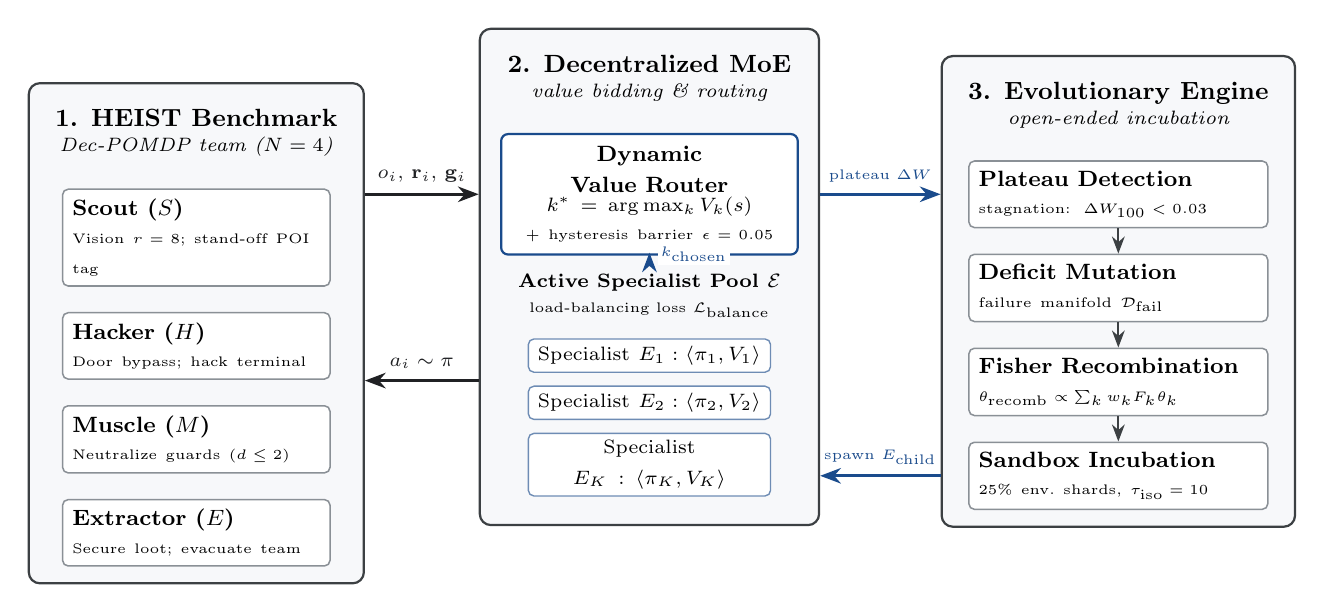
\begin{tikzpicture}[
    font=\small,
    >=Stealth,
    node distance=0.32cm,
    card/.style={
        draw=accentblue,
        fill=cardbg,
        rounded corners=2.5pt,
        line width=0.8pt,
        align=center,
        inner sep=4.5pt
    },
    rolebox/.style={
        draw=cardborder,
        fill=cardbg,
        rounded corners=2pt,
        line width=0.55pt,
        align=left,
        inner sep=3.5pt,
        text width=3.15cm
    },
    evobox/.style={
        draw=cardborder,
        fill=cardbg,
        rounded corners=2pt,
        line width=0.55pt,
        align=left,
        inner sep=3.5pt,
        text width=3.55cm
    },
    expertbox/.style={
        draw=accentsoft,
        fill=white,
        rounded corners=2pt,
        line width=0.5pt,
        align=center,
        inner sep=2.5pt,
        text width=2.9cm
    },
    flowlabel/.style={
        font=\scriptsize,
        text=textdark,
        fill=white,
        inner sep=1.2pt
    },
    flowlabelA/.style={
        flowlabel,
        text=accentblue
    }
]

% =========================================================================
% COLUMN 1: HEIST Benchmark & Roles
% =========================================================================
\node[rolebox] (scout) {
    \textbf{\footnotesize Scout ($S$)}\\[-1pt]
    \tiny Vision $r=8$; stand-off POI tag
};
\node[rolebox, below=of scout] (hacker) {
    \textbf{\footnotesize Hacker ($H$)}\\[-1pt]
    \tiny Door bypass; hack terminal
};
\node[rolebox, below=of hacker] (muscle) {
    \textbf{\footnotesize Muscle ($M$)}\\[-1pt]
    \tiny Neutralize guards ($d \le 2$)
};
\node[rolebox, below=of muscle] (extractor) {
    \textbf{\footnotesize Extractor ($E$)}\\[-1pt]
    \tiny Secure loot; evacuate team
};

\node[above=0.28cm of scout, align=center] (col1_title) {
    \textbf{\small 1. HEIST Benchmark}\\[-2pt]
    {\scriptsize\itshape Dec-POMDP team ($N=4$)}
};

\begin{scope}[on background layer]
    \node[draw=panelborder, fill=panelbg, rounded corners=4pt, line width=0.8pt,
          inner sep=6pt, fit=(col1_title)(scout)(extractor)] (panel_env) {};
\end{scope}

% =========================================================================
% COLUMN 2: Decentralized Router & Specialist Pool
% =========================================================================
\node[card, right=2.15cm of scout, yshift=0.55cm, text width=3.45cm] (router) {
    \textbf{\footnotesize Dynamic Value Router}\\[-1pt]
    \scriptsize $k^* = \arg\max_k V_k(s)$\\[-1pt]
    \tiny + hysteresis barrier $\epsilon = 0.05$
};

\node[expertbox, below=1.05cm of router] (e1) {
    \scriptsize Specialist $E_1: \langle \pi_1, V_1 \rangle$
};
\node[expertbox, below=0.16cm of e1] (e2) {
    \scriptsize Specialist $E_2: \langle \pi_2, V_2 \rangle$
};
\node[expertbox, below=0.16cm of e2] (ek) {
    \scriptsize Specialist $E_K: \langle \pi_K, V_K \rangle$
};

\node[above=0.14cm of e1, align=center] (pool_title) {
    \textbf{\scriptsize Active Specialist Pool $\mathcal{E}$}\\[-2pt]
    {\tiny load-balancing loss $\mathcal{L}_{\mathrm{balance}}$}
};

\begin{scope}[on background layer]
    \node[draw=accentsoft, fill=white, rounded corners=3pt, line width=0.55pt,
          inner sep=4pt, fit=(pool_title)(e1)(ek)] (pool_box) {};
\end{scope}

\node[above=0.28cm of router, align=center] (col2_title) {
    \textbf{\small 2. Decentralized MoE}\\[-2pt]
    {\scriptsize\itshape value bidding \& routing}
};

\begin{scope}[on background layer]
    \node[draw=panelborder, fill=panelbg, rounded corners=4pt, line width=0.8pt,
          inner sep=6pt, fit=(col2_title)(router)(pool_box)] (panel_router) {};
\end{scope}

% =========================================================================
% COLUMN 3: Evolutionary Engine (THIEF Core)
% =========================================================================
\node[evobox, right=2.15cm of router] (plateau) {
    \textbf{\footnotesize Plateau Detection}\\[-1pt]
    \tiny stagnation: $\Delta W_{100} < 0.03$
};
\node[evobox, below=of plateau] (deficit) {
    \textbf{\footnotesize Deficit Mutation}\\[-1pt]
    \tiny failure manifold $\mathcal{D}_{\mathrm{fail}}$
};
\node[evobox, below=of deficit] (fisher) {
    \textbf{\footnotesize Fisher Recombination}\\[-1pt]
    \tiny $\theta_{\mathrm{recomb}} \propto \sum_k w_k F_k \theta_k$
};
\node[evobox, below=of fisher] (incubate) {
    \textbf{\footnotesize Sandbox Incubation}\\[-1pt]
    \tiny $25\%$ env.\ shards, $\tau_{\mathrm{iso}}=10$
};

\node[above=0.28cm of plateau, align=center] (col3_title) {
    \textbf{\small 3. Evolutionary Engine}\\[-2pt]
    {\scriptsize\itshape open-ended incubation}
};

\begin{scope}[on background layer]
    \node[draw=panelborder, fill=panelbg, rounded corners=4pt, line width=0.8pt,
          inner sep=6pt, fit=(col3_title)(plateau)(incubate)] (panel_evo) {};
\end{scope}

% =========================================================================
% INTER-PANEL FLOWS (labels sit in the inter-panel gaps, on white knockouts)
% =========================================================================
% 1. Environment -> Router: observations
\draw[->, line width=1.0pt, draw=textdark]
    (panel_env.east |- router.center) -- (panel_router.west |- router.center)
    node[midway, above=2.5pt, flowlabel] {$o_i,\, \mathbf{r}_i,\, \mathbf{g}_i$};

% 2. Router -> Pool: chosen specialist (internal, within panel 2)
\draw[->, line width=0.9pt, draw=accentblue]
    (router.south) -- (pool_box.north)
    node[midway, right=2.5pt, flowlabelA, font=\tiny] {$k_{\mathrm{chosen}}$};

% 3. Pool -> Environment: actions (bottom corridor)
\draw[->, line width=1.0pt, draw=textdark]
    (panel_router.west |- pool_box.center) -- (panel_env.east |- pool_box.center)
    node[midway, above=2.5pt, flowlabel] {$a_i \sim \pi$};

% 4. Router -> Evolutionary engine: plateau trigger (top corridor)
\draw[->, line width=1.0pt, draw=accentblue]
    (panel_router.east |- plateau.center) -- (panel_evo.west |- plateau.center)
    node[midway, above=2.5pt, flowlabelA, font=\tiny] {plateau $\Delta W$};

% 5. Evolutionary engine -> Pool: spawned child (bottom corridor)
\draw[->, line width=1.0pt, draw=accentblue]
    (panel_evo.west |- incubate.center) -- (panel_router.east |- incubate.center)
    node[midway, above=2.5pt, flowlabelA, font=\tiny] {spawn $E_{\mathrm{child}}$};

% 6. Internal evolutionary flow arrows
\draw[->, line width=0.7pt, draw=panelborder] (plateau.south) -- (deficit.north);
\draw[->, line width=0.7pt, draw=panelborder] (deficit.south) -- (fisher.north);
\draw[->, line width=0.7pt, draw=panelborder] (fisher.south) -- (incubate.north);

\end{tikzpicture}
\end{document}
